% GNUPLOT: LaTeX picture with Postscript
\begingroup
  \makeatletter
  \providecommand\color[2][]{%
    \GenericError{(gnuplot) \space\space\space\@spaces}{%
      Package color not loaded in conjunction with
      terminal option `colourtext'%
    }{See the gnuplot documentation for explanation.%
    }{Either use 'blacktext' in gnuplot or load the package
      color.sty in LaTeX.}%
    \renewcommand\color[2][]{}%
  }%
  \providecommand\includegraphics[2][]{%
    \GenericError{(gnuplot) \space\space\space\@spaces}{%
      Package graphicx or graphics not loaded%
    }{See the gnuplot documentation for explanation.%
    }{The gnuplot epslatex terminal needs graphicx.sty or graphics.sty.}%
    \renewcommand\includegraphics[2][]{}%
  }%
  \providecommand\rotatebox[2]{#2}%
  \@ifundefined{ifGPcolor}{%
    \newif\ifGPcolor
    \GPcolortrue
  }{}%
  \@ifundefined{ifGPblacktext}{%
    \newif\ifGPblacktext
    \GPblacktexttrue
  }{}%
  % define a \g@addto@macro without @ in the name:
  \let\gplgaddtomacro\g@addto@macro
  % define empty templates for all commands taking text:
  \gdef\gplbacktext{}%
  \gdef\gplfronttext{}%
  \makeatother
  \ifGPblacktext
    % no textcolor at all
    \def\colorrgb#1{}%
    \def\colorgray#1{}%
  \else
    % gray or color?
    \ifGPcolor
      \def\colorrgb#1{\color[rgb]{#1}}%
      \def\colorgray#1{\color[gray]{#1}}%
      \expandafter\def\csname LTw\endcsname{\color{white}}%
      \expandafter\def\csname LTb\endcsname{\color{black}}%
      \expandafter\def\csname LTa\endcsname{\color{black}}%
      \expandafter\def\csname LT0\endcsname{\color[rgb]{1,0,0}}%
      \expandafter\def\csname LT1\endcsname{\color[rgb]{0,1,0}}%
      \expandafter\def\csname LT2\endcsname{\color[rgb]{0,0,1}}%
      \expandafter\def\csname LT3\endcsname{\color[rgb]{1,0,1}}%
      \expandafter\def\csname LT4\endcsname{\color[rgb]{0,1,1}}%
      \expandafter\def\csname LT5\endcsname{\color[rgb]{1,1,0}}%
      \expandafter\def\csname LT6\endcsname{\color[rgb]{0,0,0}}%
      \expandafter\def\csname LT7\endcsname{\color[rgb]{1,0.3,0}}%
      \expandafter\def\csname LT8\endcsname{\color[rgb]{0.5,0.5,0.5}}%
    \else
      % gray
      \def\colorrgb#1{\color{black}}%
      \def\colorgray#1{\color[gray]{#1}}%
      \expandafter\def\csname LTw\endcsname{\color{white}}%
      \expandafter\def\csname LTb\endcsname{\color{black}}%
      \expandafter\def\csname LTa\endcsname{\color{black}}%
      \expandafter\def\csname LT0\endcsname{\color{black}}%
      \expandafter\def\csname LT1\endcsname{\color{black}}%
      \expandafter\def\csname LT2\endcsname{\color{black}}%
      \expandafter\def\csname LT3\endcsname{\color{black}}%
      \expandafter\def\csname LT4\endcsname{\color{black}}%
      \expandafter\def\csname LT5\endcsname{\color{black}}%
      \expandafter\def\csname LT6\endcsname{\color{black}}%
      \expandafter\def\csname LT7\endcsname{\color{black}}%
      \expandafter\def\csname LT8\endcsname{\color{black}}%
    \fi
  \fi
  \setlength{\unitlength}{0.0500bp}%
  \begin{picture}(7200.00,5040.00)%
    \gplgaddtomacro\gplbacktext{%
      \csname LTb\endcsname%
      \put(1386,704){\makebox(0,0)[r]{\strut{} 11.5}}%
      \put(1386,1213){\makebox(0,0)[r]{\strut{} 12}}%
      \put(1386,1722){\makebox(0,0)[r]{\strut{} 12.5}}%
      \put(1386,2231){\makebox(0,0)[r]{\strut{} 13}}%
      \put(1386,2740){\makebox(0,0)[r]{\strut{} 13.5}}%
      \put(1386,3249){\makebox(0,0)[r]{\strut{} 14}}%
      \put(1386,3758){\makebox(0,0)[r]{\strut{} 14.5}}%
      \put(1386,4267){\makebox(0,0)[r]{\strut{} 15}}%
      \put(1386,4776){\makebox(0,0)[r]{\strut{} 15.5}}%
      \put(1518,484){\makebox(0,0){\strut{} 0.004}}%
      \put(2198,484){\makebox(0,0){\strut{} 0.005}}%
      \put(2878,484){\makebox(0,0){\strut{} 0.006}}%
      \put(3558,484){\makebox(0,0){\strut{} 0.007}}%
      \put(4238,484){\makebox(0,0){\strut{} 0.008}}%
      \put(4918,484){\makebox(0,0){\strut{} 0.009}}%
      \put(5598,484){\makebox(0,0){\strut{} 0.01}}%
      \put(6278,484){\makebox(0,0){\strut{} 0.011}}%
      \put(6958,484){\makebox(0,0){\strut{} 0.012}}%
      \put(484,2740){\rotatebox{90}{\makebox(0,0){\strut{}$\ln(p)$}}}%
      \put(4238,154){\makebox(0,0){\strut{}$1/T~[\si{1/\celsius}]$}}%
    }%
    \gplgaddtomacro\gplfronttext{%
      \csname LTb\endcsname%
      \put(5971,4603){\makebox(0,0)[r]{\strut{}'messung1.dat' u (1/$1):(log($2))}}%
      \csname LTb\endcsname%
      \put(5971,4383){\makebox(0,0)[r]{\strut{}'messung2.dat' u (1/$1):(log($2))}}%
    }%
    \gplbacktext
    \put(0,0){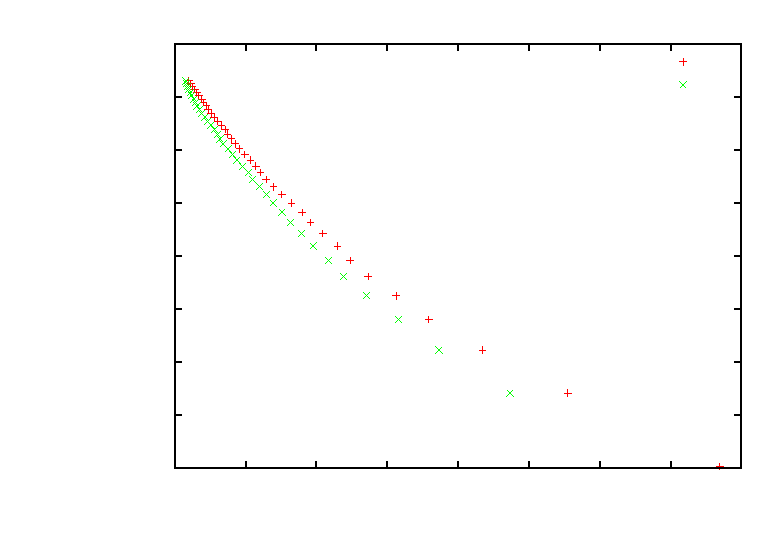
\includegraphics{Druckkurve}}%
    \gplfronttext
  \end{picture}%
\endgroup
